\section{Datenbankschema}
\label{kap:dbschema}
In diesem Kapitel werden die Anforderungen an das Datenbankschema beschrieben. Anschliessend wird ein vereinfachtes Domänenmodell vorgestellt, das als Grundlage für die weiteren Kapitel dient. Danach folgen die Beschreibung der Lösungsansätze und deren Umsetzung. Diese bildet die Grundlage für die Erläuterungen des Kapitel~\ref{kap:vfs} -~\ref{kap:lsp}.

\subsection{Anforderungen}
\label{abb:anforderungen}
Das Ziel dieser Bachelorarbeit ist die Entwicklung einer generischen, datenmodellgetriebenen Anwendung zur Verwaltung von IoT-Konfigurationen. Die Anwendungslogik soll dabei vollständig aus einem definierten Datenmodell abgeleitet werden, sodass Anpassungen im Quellcode vermieden werden. Daraus ergeben sich drei Anforderungen an das Datenbankschema: Erstens müssen Einstiegspunkte im Schema definiert werden, damit die Anwendung erkennt, wo der Verwaltungsprozess beginnt. Zweitens muss das Schema zusätzliche Validierungen unterstützen, da die verwendete Datenbanktechnologie Selva nur grundlegende Datentyp-Prüfungen bereitstellt. Drittens soll es möglich sein, zusätzliche Informationen wie beispielsweise Blattknoten oder potenzielle zyklische Verweise aus dem Schema abzuleiten, ohne dass diese im Schema definiert werden müssen.

\subsection{Domänenmodell}
\label{abb:domaenenmodell}
Das in Abschnitt~\ref{abb:tech} beschriebene Domänenmodell ist zu komplex, um es unverändert in der entwickelten Lösung zu verwenden. Deshalb wird zunächst ein vereinfachtes Modell definiert, das für die Umsetzung geeignet ist. Die Übertragbarkeit auf das Domänenmodell der Monidas-Plattform wird in Kapitel~\ref{kap:eva} untersucht.

Das für diese Arbeit verwendete Domänenmodell bildet ein typisches Szenario aus dem E-Commerce-Bereich ab. Das Modell besteht aus den fünf Entitäten: \textit{Customer}, \textit{Address}, \textit{Order}, \textit{LineItem} und \textit{Product}. Ein \textit{Customer} (Kunde) verfügt über Angaben wie Vorname, Nachname und eine E-Mail-Adresse. Jeder Kunde besitzt mehrere Adressen (\textit{Address}) und kann mehrere Bestellungen (\textit{Order}) tätigen. Eine Adresse umfasst die Strasse, Stadt sowie das Land und gehört eindeutig zu einem Kunden. Jede Bestellung besitzt eine Rechnungsadresse (\textit{billingAddress}) und optional eine Lieferadresse (\textit{shippingAddress}). Eine Bestellung besteht aus mindestens einer Bestellposition (\textit{LineItem}), welche jeweils ein Produkt (\textit{Product}) mit einer definierten Menge und einem Einzelpreis referenziert. Ein Produkt enthält eine eindeutige Beschreibung sowie einen Preis.

\begin{figure}[H]
    \centering
    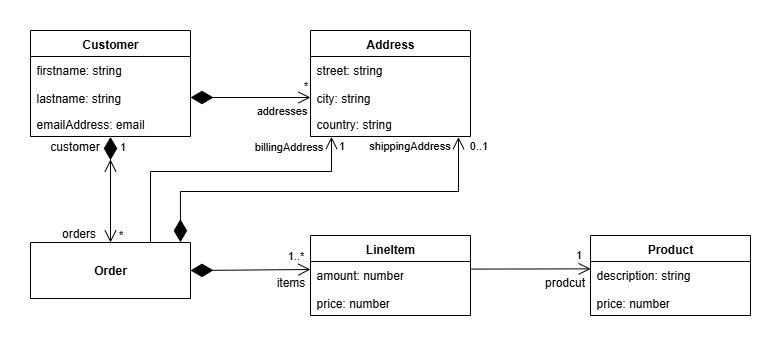
\includegraphics[width=0.8\linewidth]{Bsp_UML.png}
    \caption{Vereinfachtes Domänenmodell im E-Commerce-Kontext}
    \label{fig:uml_domaenenmodell}
\end{figure}

\subsection{Schemaerweiterungen}
\label{ab:con}
\subsubsection{Roots}
Unter dem Begriff Roots werden die im Schema definierten Einstiegspunkte verstanden. Diese bestimmen, bei welchen Entitäten die Navigation im virtuellen Filesystem beginnt. Für jeden Root wird ein Label festgelegt, das im Filesystem als Ordnername angezeigt wird. Dieses Label wird direkt im Schema definiert und kann unabhängig vom Namen der Entität frei gewählt werden.

Im E-Commerce-Domänenmodell (siehe Abbildung \ref{fig:uml_domaenenmodell}) könnten beispielsweise die Entitäten \textit{Customer} mit dem Label \textit{Customers} und \textit{Product} mit dem Label \textit{Products} als Roots definiert werden.

\subsubsection{Constraints}
Unter Constraints werden in dieser Thesis Bedingungen verstanden, die das Standardverhalten der Applikation gezielt ergänzen oder einschränken. Sie stellen sicher, dass die Daten bestimmte Anforderungen erfüllen und inhaltlich konsistent bleiben. Diese Bedingungen werden ausschliesslich von der Anwendungslogik geprüft und nicht von der Datenbank selbst.

Das Standardverhalten der Applikation sieht vor, dass neue Objekte direkt innerhalb ihres übergeordneten Knotens erstellt werden. Dieses Verhalten folgt einer Parent-Child-Hierarchie. Das Referenzieren eines bereits bestehenden Objekts ist standardmässig deaktiviert. Mit „Referenzieren“ wird in dieser Arbeit verstanden, dass beispielsweise bei einer Bestellung keine neue Adresse erstellt, sondern eine bereits existierende Adresse zugeordnet wird.

Werden jedoch zusätzliche Bedingungen benötigt, um das Standardverhalten gezielt zu erweitern, stehen die folgenden Constraints zur Verfügung: Pflichtfeld (notNull), bidirektionale Verknüpfung (bidirektional), Verbot der Erstellung neuer Objekte (denyCreation) und Erlaubnis zum Referenzieren bestehender Objekte (allowReference). Zur Veranschaulichung dieser Constraints dient folgendes Beispiel aus dem E-Commerce-Domänenmodell:

Beim Erstellen eines neuen Kunden ist die Angabe einer E-Mail-Adresse zwingend erforderlich (notNull), andernfalls ist das Speichern nicht möglich. Anschliessend erstellt der Kunde zwei Adressen, beispielsweise eine Heimadresse und eine Arbeitsadresse, welche eindeutig diesem Kunden zugeordnet sind. Möchte der Kunde eine Bestellung tätigen, ist dafür zwingend die Angabe einer Rechnungsadresse (billingAddress) erforderlich (notNull). Innerhalb der Bestellung ist das Erstellen einer neuen Rechnungsadresse technisch nicht möglich, da dies explizit deaktiviert wurde (denyCreation). Stattdessen muss eine bereits vorhandene Adresse ausgewählt werden (allowReference), beispielsweise die zuvor erstellte Arbeitsadresse. Darüber hinaus muss jede Bestellung mindestens eine Bestellposition enthalten (notNull). Diese Bestellposition wird direkt im Kontext der Bestellung erstellt und muss zwingend auf ein bereits bestehendes Produkt (Product) verweisen (allowReference, denyCreation). Optional kann zudem eine Lieferadresse angegeben werden. Diese Lieferadresse wird direkt im Kontext der Bestellung erstellt und existiert ausschliesslich dort. Das Referenzieren bereits bestehender Adressen, beispielsweise der Heim- oder Arbeitsadresse, ist hierbei technisch deaktiviert und daher nicht möglich (Standardverhalten).

\subsubsection{Dynamische Ableitung}
Die zuvor beschriebenen Schemaerweiterungen wie Constraints und Roots werden statisch im Datenbankschema definiert. Bereits während der Entwicklung zeigt sich jedoch, dass nicht jede 
Informationen  zwingend im Schema definiert werden muss. 

Mittels einer Analyse des Schemas durch geeignete Traversierungsalgorithmen lassen sich zusätzliche Informationen ermitteln, ohne diese  im Schema definieren zu müssen. Dies reduziert den Entwicklungsaufwand erheblich und schafft zugleich eine  Grundlage für spätere Erweiterungen.  Daraus ergibt sich ein dynamisch erweiterbares Schema, das flexibel auf zukünftige Anforderungen reagiert.

Das definierte Datenbankschema bildet durch die Referenzen auf andere Entitäten einen gerichteten Graphen ab. Abhängig vom Domänenmodell und der konkreten Definition des Schemas können dabei auch Zyklen vorkommen. Für eine Analyse ist es erforderlich, dass jeder Knoten im Schema mindestens einmal besucht wird, um alle Informationen ableiten zu können die benötigt werden.




Aus diesem Grund wird der Traversierungsalgorithmus der Tiefensuche (Depth-First Search, DFS) ausgewählt. Die Tiefensuche ermöglicht es, ausgehend von definierten Einstiegspunkten, jeden erreichbaren Knoten systematisch zu besuchen und potenzielle Zyklen zu erkennen. Durch dieses Vorgehen ist gewährleistet, dass sämtliche Referenzpfade im Schema vollständig analysiert werden. Dies bildet die methodische Grundlage für die anschliessende Ableitung zusätzlicher Informationen.








\subsubsection{Schema Analyse}
Die Laufzeiterweiterung des Schemas verfolgt das Ziel, zusätzliche Informationen aus dem definierten Datenmodell abzuleiten. Hierfür wird das Schema mithilfe geeigneter Traversierungsalgorithmen analysiert, um spezifische Eigenschaften zu ermitteln, welche später für die Navigation im virtuellen Filesystem und für die Validierung im Language Server verwendet werden können.


\subsubsection{Ableitung zusätzlicher Informationen}

\subsection{Bereitstellung und Zugriff}



\subsection{Umsetzung}
\subsubsection{Roots und Constraints}
In diesem Abschnitt wird erläutert, wie die zuvor beschriebenen Schemaerweiterungen „Roots“ und „Constraints“ konkret umgesetzt wurden. Da die Felder für „Roots“ und „Constraints“ in der ursprünglichen TypeScript-Typdefinition von \texttt{@colombalink/based-db-schema} nicht vorhanden sind, musste die bestehende Typdefinition erweitert werden.


Für die konkrete Umsetzung wurde das bestehende Schema aus der Colombalink-Bibliothek angepasst. Dabei wurde der ursprüngliche Typ (Schema) erweitert, um die Definition von Roots und Constraints zu ermöglichen. Die dafür notwendigen TypeScript-Features wie Omit, Intersection Types, Union Types und Generics stellten sicher, dass diese Erweiterung typsicher umgesetzt werden konnte~\cite{typescript:handbook}. Das Ergebnis ist ein erweitertes Schema, das den Anforderungen aus Abschnitt~\ref{abb:anforderungen} entspricht. Die genaue technische Umsetzung befindet sich im Anhang in Listing~\ref{lst:extended-schema}.

Im vorherigen Abschnitt wurde bereits erläutert, wie im konkreten E-Commerce-Domänen\-modell die Entitäten \textit{Customer} und \textit{Product} als Roots definiert wurden, sowie welche Constraints für die Entität \textit{Order} gesetzt wurden. Im nachfolgenden Listing~\ref{lst:con} ist nun dargestellt, wie diese Definitionen konkret in der erweiterten Typdefinition gesetzt werden:

\newpage
\lstinputlisting[
caption={Definition von Roots und Constraints im erweiterten Schema},
label={lst:con},
style=customtypescript
]{listings/con.json}

Damit bildet das erweiterte Schema die zuvor beschriebenen fachlichen Anforderungen vollständig ab.


\subsubsection{Laufzeit Erweiterung}